\chapter{Data Structures}
\section{Data Types}
\subsection{Primative Types}

\rsrc{Primatives} \href{https://en.wikipedia.org/wiki/Primitive_data_type}{Wiki Link}

These are the basic elements:
	\begin{enumerate}
		\item Bool
		\item char
		\item float
		\item double
		\item int
		\item string
		\item reference
		\item enum
	\end{enumerate}

\subsection{Composite Types}

\rsrc{Composites}\href{https://en.wikipedia.org/wiki/Composite_data_type}{Wiki Link}


\subsection{Abstract Data Types}

\rsrc{Abstract Types}\href{https://en.wikipedia.org/wiki/Abstract_data_type}{Wiki Link}

\subsection{Linear Data Structures}



\section{Abstract Data Types}
Abstract data types (ADT) \ra its only a data structure if you're talking about the implimentation.

\subsection{Trees}

	\rsrc{Tree}\href{https://en.wikipedia.org/wiki/Tree_(data_structure)}{Wiki Link}
	
	A tree is a data structure made up of nodes connected by edges without having a cycle in it (a node cannot call itself in anyway). A linear list is a trivial tree.

\begin{table}
	\begin{tabular}{r p{.8\textwidth}}
		Nodes&A vertex connected to other vertexes by edges, in a tree nodes are connected by edges\\
		Edge&Connections to other nodes\\
		Subtrees&A connected group of children nodes connected to a parentthats not the root\\
		Digraph&\\
		Root& Top node of a tree\\
		Child&A node directly connected to another, away from the root\\
		Parent&Directly connected node towards the root. Can only have 1 parent as this causes cycles.\\
		Sibling&Node with same parent\\
		Decendant&Node accessible by parent to child\\
		Ancestor&Node accessible by traversing child to parent\\
		Leaf&(or external node) A node with no children (degree 1)\\
		Branch&(or internal node) A node with children (degree $>$1)\\
		Degree&The number of edges on a nodes\\
		Path&Sequence of nodes and edges to reach another node\\
		Level&1+connections to root of a node. (R)-( )-( )-(A) A has level4.\\
		Node Height&Number of edges on the longest path between that node and a leaf.\\
		Depth&Number of edges from the root to a given node\\
		Forest&A set of disjointed trees\\
		Branching Factor&Maximum number of children per node\\

	\end{tabular}
\end{table}

\subsubsection{Search Tree}

\rsrc{Search Tree}\href{https://en.wikipedia.org/wiki/Search_tree}{Wiki Link}

Tree data structure used for locating specific keys from within a set. Needs to be relatively balanced to be efficient.

\subsubsection{Binary Trees}

\rsrc{Binary Trees}\href{http://www.allisons.org/ll/AlgDS/Tree/}{Allisons Link}\\
\rsrc{Binary Trees}\href{https://en.wikipedia.org/wiki/Binary_tree}{Wiki Link}


\subsection{Hash Tree}

\rsrc{Hash Array Tree}\href{https://en.wikipedia.org/wiki/Hashed_array_tree}{Wiki Link}

\rsrc{Merkle Tree}\href{https://en.wikipedia.org/wiki/Merkle_tree}{Wiki Link}

\subsection{Trie}

\rsrc{Trie}\href{https://en.wikipedia.org/wiki/Trie}{Wiki Link}

Type of search tree. No node stores the key associated with its node, the position in the tree decides its key. All of the decendants of a node have the same prefix, the root is an empty string.

Commonly used for autocomplete and predictive text. 

A trie can replace hash table:
\begin{itemize}
	\item Worst case lookup is better
	\item No key collisions
	\item Buckets are only necessary if a key identifies multiple values
	\item Can provide alphabetical ordering
\end{itemize}

Drawbacks:
\begin{itemize}
	\item Tends to be slower than a hash for lookups
	\item Floats can cause nasty long search chains
	\item Can require more memory as the keys are split up instead of contiguous
\end{itemize}

\begin{table}
	\begin{tabular}{r p{.8\textwidth}}
		
	\end{tabular}
\end{table}

\begin{figure}
	\centering
	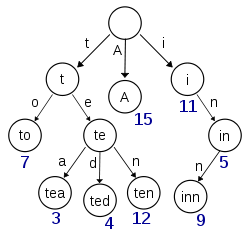
\includegraphics[width=.5\textwidth]{trie.png}
	\caption{A trie data type visualization}
\end{figure}



\subsection{Heap}

\rsrc{The Heap}\href{https://en.wikipedia.org/wiki/Heap_%28data_structure%29}{Wiki Link}

	Tree data type, subtype of a priority queue. two types \ra min and max. In a min/max heap the root is the lowest/highest value in the tree.

	The binary heap was introduced for the heap sort algorithm. The heap is partially ordered.

	\begin{itemize}
		\item Heap Property: with P \ra parent node, C \ra child node, then the key of P is ordered with respect to C. This applies for every child and parent.
		\item The root is the lowest or highest value
		\item Items always go in the next free slot. If it isnt in the right place compare to its parent and swap is the parent is smaller/larger.
	\end{itemize}


\subsection{Sets}
\rsrc{Sets}{\href{https://en.wikipedia.org/wiki/Set_(abstract_data_type)}{Wiki Link}

\section{Hashes}

Hash function 

\subsection{Hash Table}

\rsrc{Hash Table}\href{https://en.wikipedia.org/wiki/Hash_table}{Wiki Link}

Hash tables tend to be faster than other table data structures, degrading to the same average lookup time of an unordered array only in the worst case senario.
If the hash function is complex and the entry count small, this advantage can be lost.


\begin{table}
\centering
	\caption{\textbf{Time Complexity}}
\begin{tabular}{lll}
	Algo&Ave&Worst\\
	Space&O(n)&O(n)\\
	Search&O(1)&O(n)\\
	Insert&O(1)&O(n)\\
	Delete&O(1)&O(n)\\
\end{tabular}
\end{table}
A hash table is an associative array (i.e. a dictionary) that maps keys to values. 
Puts a key through a hash function to find/retrieve an index to an array of buckets
\begin{table}
	\label{table:hashTableTerms}
	\caption{Hash table terms}
	\begin{tabular}{r p{.8\textwidth}}
		Key& The name of a value/ attribute\\
		Bucket& The array elements. Typically a dynamic array\\
		Slot& Synonym for bucket\\
		Hash function& computes the index from a key\\
		Load Factor& $\frac{entries}{buckets}$ The higher the load factorthe slower the search, the lower the load facter the more memory wasted.\\
	\end{tabular}
\end{table}

\subsubsection{Collision Resolution}
\begin{tabular}{r p{.8\textwidth}}
	Separate Chaining&Buckets have a list of their own entries to a single has, if the hash matches and the key doesn't do a linear search of the list\\
	Open Addressing&On a collision, the new entry takes the next open slot. Useful if memory is an issue and the entries are smaller that $\sim$ 4$\times$ sizeof(*)\\

\end{tabular}

\subsection{Linked Lists}
\subsubsection{Singley linked lists}
\begin{center}
\begin{tikzpicture}[list/.style={rectangle split, rectangle split parts=2,
		    draw, rectangle split horizontal}, >=stealth, start chain]
			  \node[list,on chain] (A) {12};
			    \node[list,on chain] (B) {99};
				  \node[list,on chain] (C) {37};
				  \node[on chain,draw,inner sep=6pt] (D) {};
				    \draw (D.north east) -- (D.south west);
				  \draw (D.north west) -- (D.south east);
			    \draw[*->] let \p1 = (A.two), \p2 = (A.center) in (\x1,\y2) -- (B);
			  \draw[*->] let \p1 = (B.two), \p2 = (B.center) in (\x1,\y2) -- (C);
		    \draw[*->] let \p1 = (C.two), \p2 = (C.center) in (\x1,\y2) -- (D);
	\end{tikzpicture}
\end{center}
\subsubsection{Doubley linked lists}


\subsection{Queue}

\rsrc{Queue}\href{https://en.wikipedia.org/wiki/Queue_(abstract_data_type)}{Wiki Link}

Fifo, any added item are added to the end/tail of the structure (inqueued). Items are only removed from the front/head (dequeued). 

\begin{itemize}
	\item Simulate waiting lines
	\item Buffers for I/O
\end{itemize}
\subsection{Priority Queue}
	
	\subsection{Stack}

	\rsrc{The Stack}\href{https://en.wikipedia.org/wiki/Stack_(abstract_data_type)}{Wiki Link}

	Opposite of a queue \ra LIFO


\subsection{Ring Buffer}

\rsrc{Ring Buffer}\href{https://en.wikipedia.org/wiki/Circular_buffer}{Wiki Link}

\subsubsection{Union}
	\subsubsection{Tagged Union}



